\chapter{Control Overhead} \label{CHAP:CTLOVERHEAD}

[WIP]

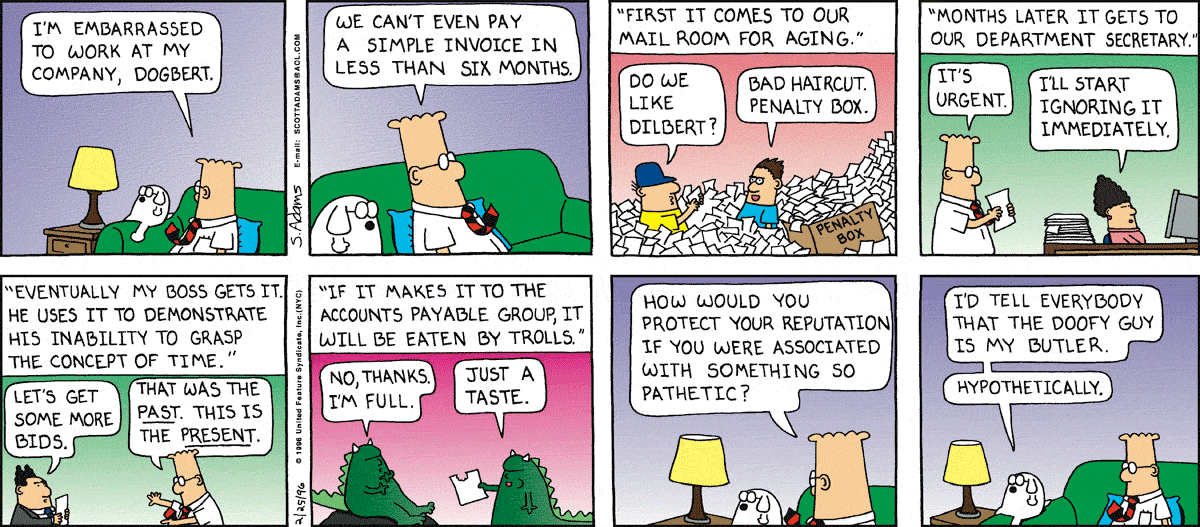
\includegraphics[width=\textwidth]{images/chap6/dilbert.png}

\section{What is Control Overhead?}

If a modern CPU processes a network message it goes through different layers of mediation.  The device, for example, an Ethernet adaptor, \textit{interrupts} the CPU, asking somewhat
stridently for attention. Control is passed to the kernel. The kernel batches interrupts wherever possible, does the network layer processing for the packet, and finally \textit{schedules} the application process (say, a Web server) to run. The web server creates new processes/threads, read/write files (\textit{system call}) and sends out the HTTP response by writing to the corresponding connection (another system call).

Thus an unoptimized implementation can incur considerable process-switching overhead
(hundreds of microseconds) if the application and networking code is poorly structured. Even
if process-structuring overhead is removed, system calls can cost tens of microseconds, and
interrupts can cost microseconds. To put these numbers in perspective, observe that on a 10-GB Ethernet link, a 40-byte packet can arrive at a PC every 3.2 µsec.





\section{Getting Rid of Control Overhead}

This section describes how to reduce control overhead costs, from the largest (context switches) to the smallest (interrupt overhead).

\subsection{Context switches}

In what follows, we will use a Web server as an example of a canonical server that may require the handling of a large number of connections. To do this efficient the server has to take every opportunity for concurrency

We now consider various ways to structure a server application and their effects on concurrency and scheduling overhead.

\subsubsection{Process per Client}

For every client the web server creates a new process. This results in the following advantages and disadvantages:

\begin{itemize}
\item[$\oplus$] OS scheduler juggles between clients
\item[$\circleddash$] process-context switching is expensive
\item[$\circleddash$] spawning a new process is also expensive
\item[$\circleddash$] matchmaking between new arriving clients and processes in pool
\end{itemize}


\subsubsection{Thread per Client}

Threads share the same virtual memory and generally trust each other, as is appropriate for all the threads processing different clients in a web server.

\begin{itemize}
\item[$\oplus$] common cache
\item[$\oplus$] smaller overhead than process per client
\item[$\circleddash$] still considerable overhead (e.g. save/restore stacks and registers)
\end{itemize}


\subsubsection{Event-Driven Scheduler}

If a general-purpose operating system facility is too expensive, the simplest strategy is to avoid
it completely. Thus while thread scheduling provides a facility for juggling between clients
without further programming, if it is too expensive, the application may benefit from doing
the juggling itself. Effectively, the application must implement its own internal scheduler that
juggles the state of each client.

\begin{center}
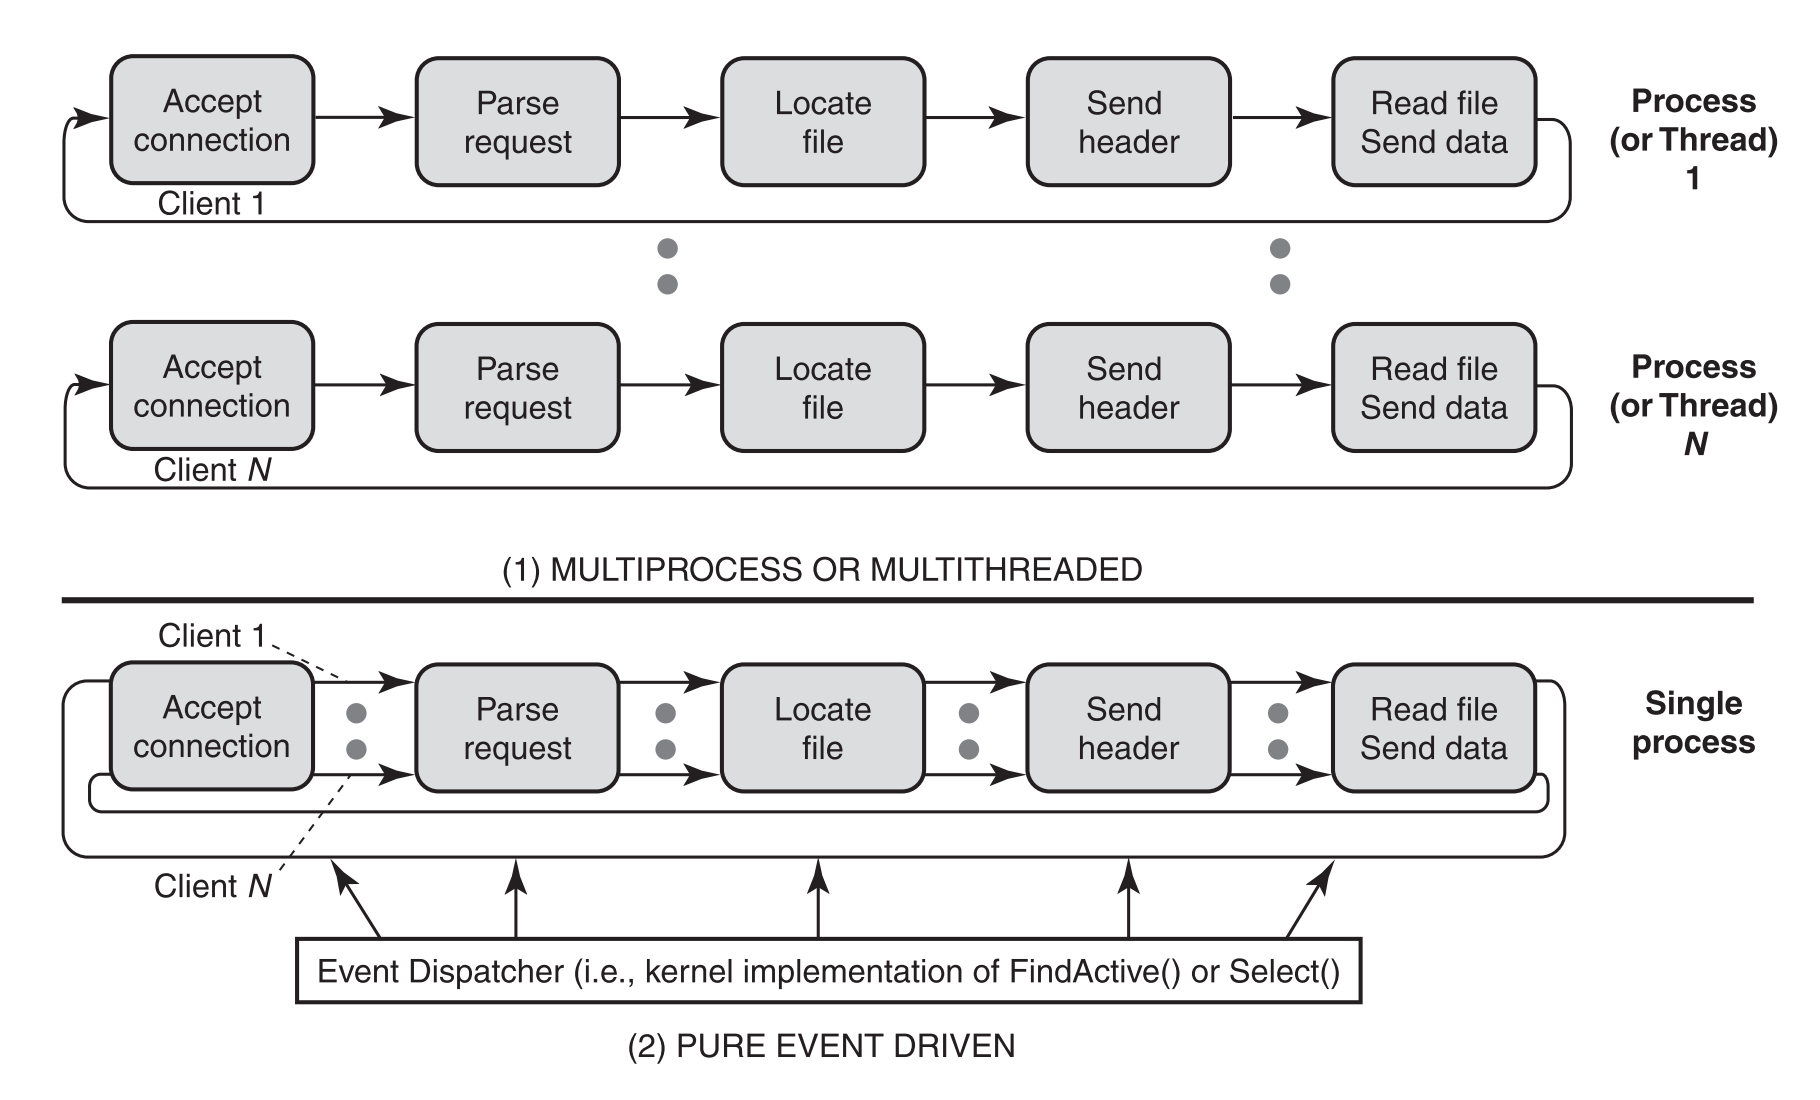
\includegraphics[width=.7\textwidth]{images/chap6/multiprocess-event.png}
\end{center}

The main idea is that the application stays in a loop invoking the FindActive()\footnote{This is a generic term. e.g. UNIX provides the select() system call.} call, which returns a list of all completed I/O descriptors. Assuming there is always some work to do on behalf of some client, the call will return with a list of I/O descriptors (e.g., file 1 data is now in memory, connection 5 has received data) with pending work. When the Web server processes these active descriptors, it loops back to making another FindActive() call.

\begin{itemize}
\item[$\oplus$] internal scheduling is more efficient
\item[$\circleddash$] requires non-blocking disk operations
\end{itemize}


\subsubsection{Event-Driven Server with Helper Processes}

The difficulty is that many operating systems, such as Solaris and UNIX, allow nonblocking read() and write() operations on network connections but may block when used on disk
files. Thus in such operating systems one must choose between the loss of concurrency incurred by blocking on disk I/O and going beyond the single-process model.

To avoid this problem, blocking operations are outsourced to helper processes.



\subsection{System calls}

When the application wants to receive data, it must specify buffers where the received
packet data should be written to. Today, in UNIX this is typically done using system calls,
where the application tells the kernel about data it wishes to send and buffers it wishes to receive to.

This appears to be required because there can be several applications sending and receiving
data from a common adaptor; since the adaptor is a shared resource, it seems unthinkable for an application to write directly to the device registers of a network adaptor without kernel mediation to check for malicious or erroneous use. Or is it?

Analogous to memory pages, our application can allocate adaptor pages and read/write descriptors directly to them without bothering the kernel. A descriptor is a small piece of information that describes the buffer in main memory where the data for the next packet should be written to. When a new packet arrives for the web application, the adaptor will demultiplex the packet on the basis of those descriptors.


\subsection{Interrupts}

There is no way to avoid interrupts completely. However, one can reduce interrupt overhead using the following tricks.

\begin{itemize}
\item \textbf{Interrupt only for significant events} e.g. only for the first packet received in a stream of packets.

\item \textbf{Polling} CPU keeps checking to see if packets have arrived.

\item \textbf{Application controlled} The sender is able to control when the receiver interrupts by passing a bit in the packet header.
\end{itemize}
